\def\documentauthorname         {Рафаел Динев Калъчев}
\def\documentauthoremail        {kalachev.rafael@gmail.com}
\def\documenttitle              {Платформа за безпилотен летателен апарат с четири ротора}
\def\documenttitleshort         {Платформа за безпилотен летателен апарат}
\def\documentsubject            {}
\def\documentkeywords           {embeded,quadrotor,automation,microcontroller,control,drone}
\def\documenttype               {Дипломна работа}
\def\documentlocation           {Технически Университет София}
\documentclass{article}

\usepackage{xargs}

\usepackage{fontspec}
\usepackage{microtype}
\setmainfont[Ligatures={TeX,Common,Rare}]{Heuristica}

\newfontfamily{\cyrillicfonttt}{Heuristica}
\newfontfamily{\cyrillicfontsf}{Heuristica}
\newfontfamily{\englishfonttt}{Fira Code}
\usepackage{polyglossia}
\setdefaultlanguage{bulgarian}

\captionsbulgarian{
  \def\equationname{Уравнение}%
  \def\footnotename{Бележка}%
  \def\itemname{Точка}%
  \def\figurename{Фигура}%
  \def\tablename{Таблица}%
  \def\partname{Част}%
  \def\appendixname{Апендикс}%
  \def\chaptername{Глава}%
  \def\sectionname{Секция}%
  \def\subsectionname{Събсекция}%
  \def\subsubsectionname{Събсъбсекция}%
  \def\paragraphname{Параграф}%
  \def\subparagraphname{Събпарагра}%
  \def\FancyVerbLinename{Линия}%
  \def\theoremname{Теорема}%
  \def\pagename{Страница}%
}

\makeatletter
\ifdefined\HyLang@bulgarian\else
\gappto\blockextras@bulgarian{%
  \def\equationautorefname{Уравнение}%
  \def\footnoteautorefname{Бележка}%
  \def\itemautorefname{Точка}%
  \def\figureautorefname{Фигура}%
  \def\tableautorefname{Таблица}%
  \def\partautorefname{Част}%
  \def\appendixautorefname{Апендикс}%
  \def\chapterautorefname{Глава}%
  \def\sectionautorefname{Секция}%
  \def\subsectionautorefname{Събсекция}%
  \def\subsubsectionautorefname{Събсъбсекция}%
  \def\paragraphautorefname{Параграф}%
  \def\subparagraphautorefname{Събпарагра}%
  \def\FancyVerbLineautorefname{Линия}%
  \def\theoremautorefname{Теорема}%
  \def\pageautorefname{Страница}%
}
\let\inlineextras@bulgarian\blockextras@bulgarian
\fi

\ifdefined\HyLang@english\else
\appto\blockextras@english{%
  \def\equationautorefname{Equation}%
  \def\footnoteautorefname{footnote}%
  \def\itemautorefname{item}%
  \def\figureautorefname{Figure}%
  \def\tableautorefname{Table}%
  \def\partautorefname{Part}%
  \def\appendixautorefname{Appendix}%
  \def\chapterautorefname{Chapter}%
  \def\sectionautorefname{section}%
  \def\subsectionautorefname{subsection}%
  \def\subsubsectionautorefname{subsubsection}%
  \def\paragraphautorefname{paragraph}%
  \def\subparagraphautorefname{subparagraph}%
  \def\FancyVerbLineautorefname{line}%
  \def\theoremautorefname{Тheorem}%
  \def\pageautorefname{page}%
}
% \inlineextras@english is empty, so we simply set it
% equal to \blockextras@english
\let\inlineextras@english\blockextras@english
\fi
\makeatother


\setotherlanguage{english}

\usepackage[style=german]{csquotes}
\usepackage{amsmath}
\usepackage{amsfonts}
\usepackage{amssymb}
\usepackage{amsthm}

\usepackage[colorlinks]{hyperref}

\usepackage{url}

\usepackage[ backend=biber,
             sorting=nty,
             style=ieee,
             defernumbers=false,
             dashed=false]{biblatex}

\usepackage{xcolor}

%TODO define colors

%colours

\definecolor{Plum}{rgb}{0.56, 0.27, 0.52}
\definecolor{OliveGreen}{rgb}{0,0.6,0}
\definecolor{emerald}{rgb}{0.31, 0.78, 0.47}
\definecolor{airforceblue}{rgb}{0.36, 0.54, 0.66}

%code
\definecolor{codegreen}{rgb}{0,0.6,0}
\definecolor{codegray}{rgb}{0.5,0.5,0.5}
\definecolor{codepurple}{rgb}{0.58,0,0.82}
\definecolor{backcolour}{rgb}{0.95,0.95,0.92}

%
\definecolor{unimportant}{rgb}{0.66,0.66,0.66}

\usepackage{graphicx}
\usepackage{scalerel}
\graphicspath{
    {graphics/}
    {src/}
}


\usepackage{listings}

\lstdefinestyle{octavecodestyle}{
    backgroundcolor=\color{backcolour},
    commentstyle=\color{codegreen},
    keywordstyle=\color{magenta},
    numberstyle=\tiny\color{codegray},
    stringstyle=\color{codepurple},
    basicstyle=\ttfamily\footnotesize,
    breakatwhitespace=false,
    breaklines=true,
    captionpos=b,
    keepspaces=true,
    numbers=left,
    numbersep=5pt,
    showspaces=false,
    showstringspaces=false,
    showtabs=false,
    tabsize=2
}


\lstset{style=octavecodestyle}



\usepackage{tabularx}

\usepackage[colorinlistoftodos,prependcaption,textsize=tiny]{todonotes}
\usepackage{soul}
\usepackage{easyReview}


\setreviewson
%\setreviewsoff

\newcommandx{\unsure}[2][1=]{\todo[linecolor=red,backgroundcolor=red!25,bordercolor=red,#1]{#2}}
\newcommandx{\change}[2][1=]{\todo[linecolor=blue,backgroundcolor=blue!25,bordercolor=blue,#1]{#2}}
\newcommandx{\info}[2][1=]{\todo[linecolor=OliveGreen,backgroundcolor=OliveGreen!25,bordercolor=OliveGreen,#1]{#2}}
\newcommandx{\improvement}[2][1=]{\todo[linecolor=Plum,backgroundcolor=Plum!25,bordercolor=Plum,#1]{#2}}
\newcommandx{\thiswillnotshow}[2][1=]{\todo[disable,#1]{#2}}


\usepackage[a4paper,width=140mm,top=30mm,bottom=30mm]{geometry} % TODO read on geometry

\usepackage{fancyhdr} % TODO read on fancyhdr

\usepackage[section]{placeins}

\pagestyle{fancy}

\fancyhead[L]{\scalerel*{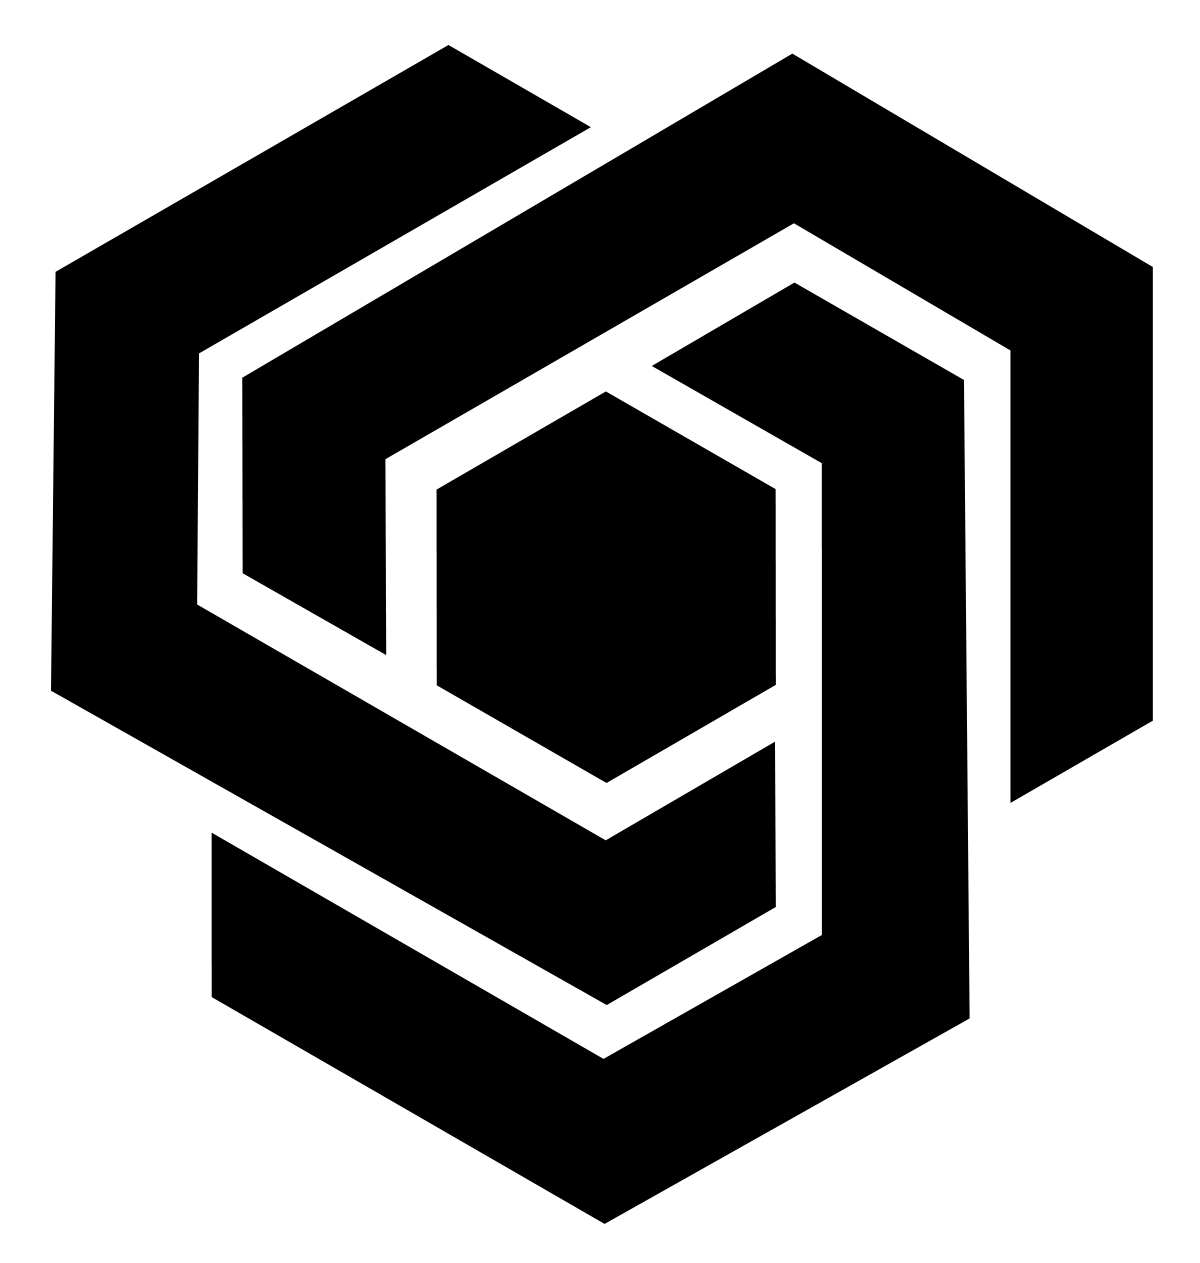
\includegraphics{logo}}{\strut}\quad{\small ТУ София}}
\fancyhead[R]{{\small \documentauthorname} }
\fancyfoot[C]{\thepage}

\renewcommand{\headrulewidth}{0pt}
\renewcommand{\footrulewidth}{0pt}


\hypersetup{
pdfauthor = {\documentauthorname},
pdftitle = {\documenttitle},
pdfsubject = {\documentsubject},
pdfkeywords = {\documentkeywords},
pdfcreator = {LuaLaTeX with hyperref package},
pdfproducer = {LuaLaTeX},
colorlinks = true,
linkcolor = red,          % color of internal links
citecolor = green,        % color of links to bibliography
filecolor = magenta,      % color of file links
urlcolor = blue,          % color of external links
}

\addbibresource{bibliography/thesis.bib}



\setlength{\parindent}{.5em}
\setlength{\parskip}{1.5em}
\linespread{1.5}



\begin{document}

\begin{titlepage}

	\center % Centre everything on the page

	%------------------------------------------------
	%	Headings
	%------------------------------------------------

    \textsc{\LARGE \textbf{\documenttype}}\\[0.2cm] % Main heading such as the name of your university/college
	\noindent\rule{16cm}{0.4pt}\\[0.2cm]
	\textsc{\Large Катедра Системи и Управление}\\[0.0cm] % Major heading such as course name
	\noindent\rule{16cm}{0.4pt}\\[0.5cm]
	\textsc{\large на тема:}\\[0.3cm] % Minor heading such as course title

	%------------------------------------------------
	%	Title
	%------------------------------------------------



	{\huge\bfseries \documenttitle }\\[0.3cm] % Title of your document



	%------------------------------------------------
	%	Author(s)
	%------------------------------------------------

	\vspace{0.5cm}

	\begin{minipage}{0.4\textwidth}
		\begin{flushleft}
			\large
			\textit{Автор:}\\
		     \textsc{Рафаел Калъчев}, \\ IV курс, № 011217071\\
		\end{flushleft}
	\end{minipage}
	~
	\begin{minipage}{0.4\textwidth}
		\begin{flushleft}
			\large
			\textit{Ръководител:}\\
			гл. ас. д-р Александър Хотмар \\[1.em]

            \textit{Ръководител на кат. СУ:}\\
            доц. д-р Теофана Пулева \\
		\end{flushleft}
	\end{minipage}

	% If you don't want a supervisor, uncomment the two lines below and comment the code above
	%{\large\textit{Author}}\\
	%John \textsc{Smith} % Your name

	%------------------------------------------------
	%	Date
	%------------------------------------------------

	\vspace{0.5cm}
	\textsc{\LARGE Технически Университет\\
        София\\[0.3cm]
        	\vspace{0.5cm}
		\large Факултет Автоматика\\
        АИУТ}\\[0.5cm]
	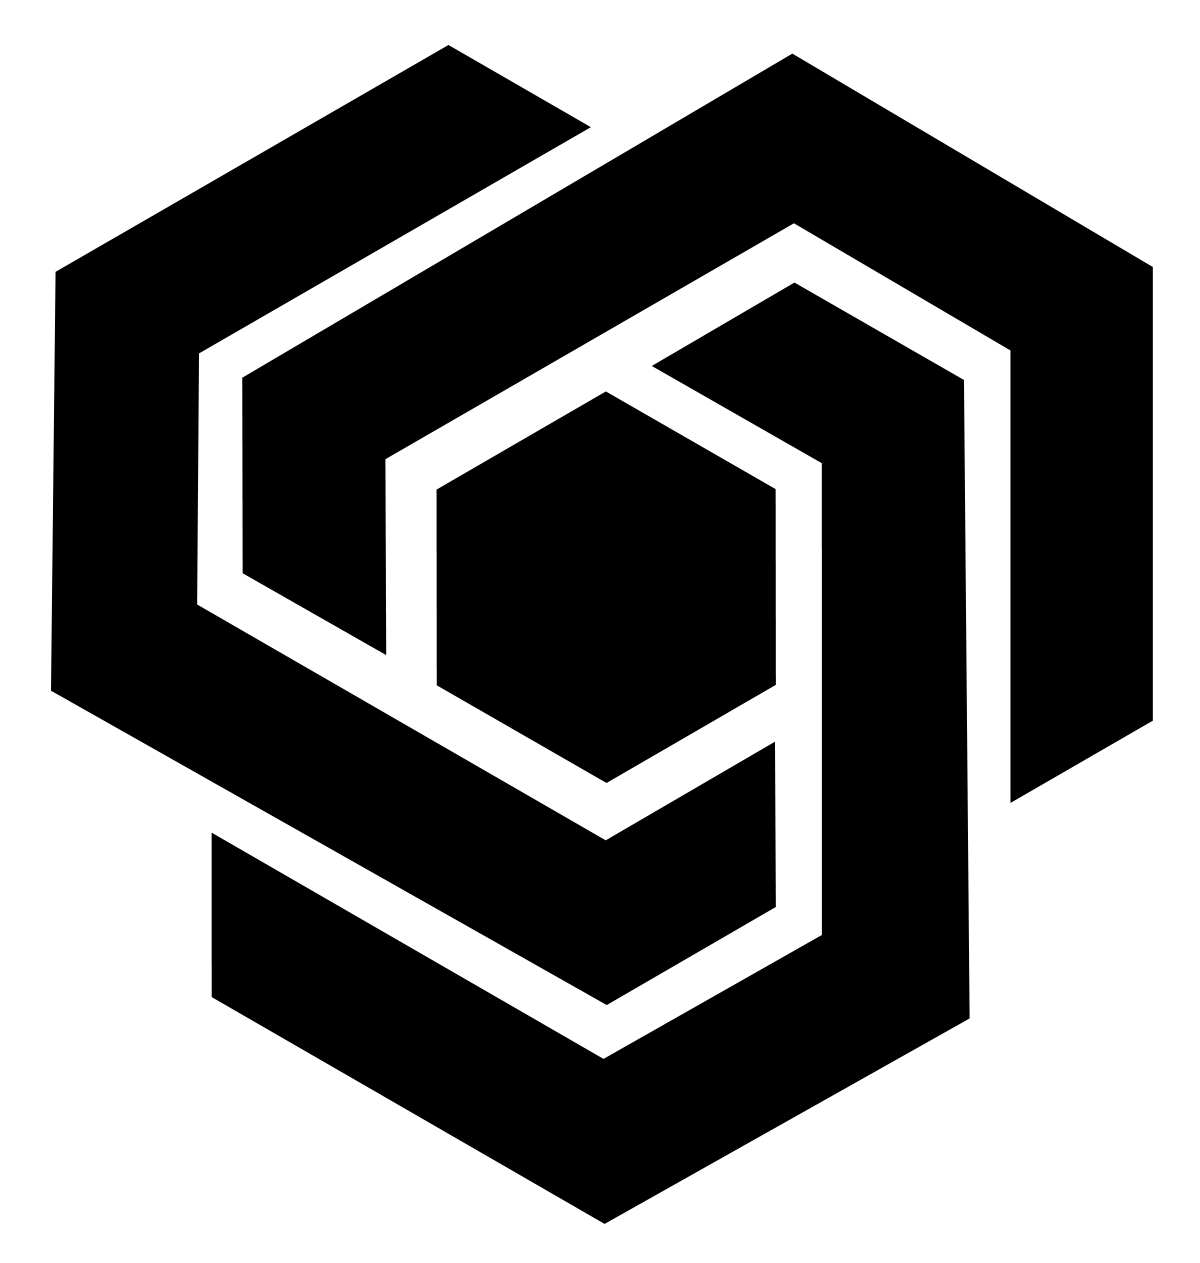
\includegraphics[width=0.35\textwidth]{logo}

	\vspace{\stretch{3}} 



        \textsc{Април, 2021\\
        София}

	%------------------------------------------------
	%	Logo
	%------------------------------------------------

	%\vfill\vfill
	%\includegraphics[width=0.2\textwidth]{placeholder.jpg}\\[1cm] % Include a department/university logo - this will require the graphicx package

	%----------------------------------------------------------------------------------------

	\vspace{\stretch{1}} % Push the date up 1/4 of the remaining page


\end{titlepage}


\tableofcontents
\listoffigures
\newpage


\section{Въведение}  

През последните години се наблюдава засилване на интереса към създаване и управление на т.нар. квадрокоптери или четирироторни хеликоптери.
Квадрокоптерът представлява малък до среден по размер безпилотен летателен апарат (UAV), който има четири симетрично разположени ротора, обикновено прикрепени в краищата на рамената на платформата. 

В сравнение с други подобни платформи четирироторният апарат притежава здравина, механична простота, стабилност и относително ниска цена, което го прави обект на внимание както по военни, така и по търговски причини.

По-голямата част от четирироторните хеликоптери са конструирани от компоненти за играчки с дистанционно управление и в резултат на това тези устройства нямат необходимата надеждност и производителност, за да бъдат практични експериментални платформи. 

Поради предимствата пред обикновените летателни апарати, потенциала по отношение употребата в открита среда и поради сложната динамика управлението на четирироторен летателен апарат е фундаметнално труден и интересен проблем.



Този труд се концентрира върху цялостното изграждане на система за управление като предоставя
за пример създаване на \enquote{Безпилотна платформа за летателен апарат с четири ротора}.
Ще се наблегне върху направата на софтуер из основи за безпилотния летателен апарат.
По този начин ще бъде демонстрирано как може да се изгради основа за софтуер за управление на непознат, иновативен микроконтролер, за който не съществуват библиотеки. 

С цел да се подобри разбирането за работата на софтуера на системата за управление, ще се елиминира интеграцията с MATLAB (за управление) и използването на специфични много популярни модули, за които има налични множество библиотеки.
Ще бъде разгледан начин за инициализиране и управление на периферията, както методи за обработка на данните, постъпващи от периферията за сформиране на управляващи въздействия.

Избраната система е многомерна и има състояния, които не могат да бъдат измервани директно.
Този труд ще демонстрира изграждането на наблюдателя на състоянията на системата, както и неговата имплементация като част от алгоритъма за управление. 


Този труд няма да разглежда изграждането на система за управление с помощта на Операционна система за реално време. 
Изграждането на ОС за реално време ще бъде плот на отделен бъдещ труд.
Работата в реално време ще бъде осигурена от софтуера на конторлера, но тя няма да бъде разпределена на отделни \enquote{задачи}, а ще се управлява от регулярните прекъсвания на таймера, съпътствани от проста логика и функции, имплементирани по начин, който ще гарантира изпълнение за определеното време.

Като част от този труд е изградена платформа за управление на ъгъл на завъртане на рамо с два ротора.
Тази задача е идентична с една от подзадачите за управление на четирироторна платформа.

\section{Използвана среда и инструменти за разработка на платформата}

\subsection{Среда за разработка на софтуера}

Изградената среда за разработка на софтуера е конфигурируема и поддрържа базата микроконтролери от семейство \textit{STM32M4xxx}.
Като основа е използвана автоматичната система за изгращане \textit{GNU make},която позволява насочена обработка на файловете изграждащи софтуера и
документацията, с цел намаляване времето за обработка. \textit{GNU make} свързва всички елементи от средата и последователно изпълнява само нужните
команди с цел намаляване на използваните ресурси. Интерфейсът е команден, което позволява допълнителни нива на автоматизиране на процесите по разработка.

За компилация е използван свободният комилатор на \textit{GNU} 
\textit{GCC (GNU Comiler Collection) ARM NON-EABI (Embedded-Application Binary Interface)}. Тази разновидност на компилатора е неспецифична към
операционна система, което е нужно, тъй като разработваният софтуер няма да работи под операционна система. Тази разновидност на комилатора също е
неспецифична към производител на процесора.
\textit{GCC ARM NON-EABI} Е колекция от свързани инстументи, за разработка на софтуер за системи с ядро \textit{ARM}.
Състои се от комилатор на езика C, асемблатор, линкер, инстументи за преглед и конверсия между стандартни формати двоични файлове.

За връзка с контролера е изполван командният пакет за \textit{ST-LINK} на \textit{STMicroelectronics}.
Пакетът предоставя команди за връзка с програматорът \textit{ST-LINK V2}, чрез който се програмира микроконтролета.
Пакетът се използва също за управление на потрът за дебъг, през който се осъществява дебъг комуникацията.

Като дебъгер е използван свободният дебъгер на \textit{GNU}
\textit{GDB}. Той може да се използва както за локално така и за отдалечено дебъгване.
Тъй като микроконтролера е отдалечен използваме командният пакет за \textit{ST-LINK} да конфигурираме порт за дебъг,
към който се свързваме чрез \textit{GDB}.

За писането на софтуера е изполван терминалният текстов редактор \textit{VIM} поради удобният си команден интерфейс.
За генериране на всички софтуерни тагове, които \textit{VIM} ще използва за подпомагане на процеса за разработка 
е използван софтуера \textit{ctags}, който обработва релевантните файлове и поддържа опростена база данни за всички индентификатори,
имена и тагове, които \textit{VIM} изпозва спрямо контекста.











\section{Използван хардуер}


\subsection{Микроконтролер}

Микроконторлерът използван за проекта е с ядро с архитектура \textit{ARM Cortex-M4}, произведен от \textit{STMicroelectronics}.
Модел \texttt{stm32f429ZIT6U}.


\subsection{Жироскоп и Акселерометръ}

\subsection{Магнитометър}


\section{Архитектура на системата}

Архитектурната част на системата е организирана в три основни части:

Първата част се отнася до дизайна на платформата (физическото оформление),
Основните концептуални идеи покрити в физическото оформление, разпределението на хардуера
и това как този хардуер ще бъде използван за управлението.
Как е свързана системата (хардуерно)

Част втора Архитектура на уравлението (помисли за това)

Част трета разглежа софтуерната архитектура на управляващото устройство.

\cite{stmcurefman} 

\subsection{Конструкция на платформата}

\subsection{Платформа с четири ротора}
\FloatBarrier

Платформата \autoref{fig:drone_construction} е конструирана от два метални П-образни профила, сключващи прав ъгъл помежду си и имащи пресечна точка в средата.
В края на профилите се намира по един безчетков постояннотоков мотор (без обратна връзка).
Перките са свързани директно (без трансмисия) за въртящата ос на моторите.
Батерията и контролният модул са позиционирани в средата на платформата.
Батерията се намира под пресечната точка на профилите.
Управляващото устройство е над пресеччната точка на профилите
върху изработена, като част от проекта, платформа.

При този начин на организиране на хардуера центърът на тежеста лежи под пресечната точка на профилите.


\begin{figure}[htpb!]
    \centering
    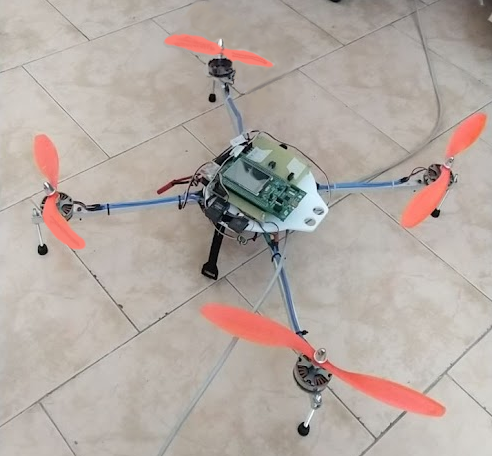
\includegraphics[width=0.5\textwidth]{drone_construction}
    \caption{Конструкция на платформата с четири ротора}
    \label{fig:drone_construction}
\end{figure}



\FloatBarrier
\subsection{Платформа за управление на ъгъл на завъртане}
\FloatBarrier

Платформата за управление на ъгъл на завъртане има за цел да ни позволи лесно и безаварийно да изпробваме алгоритмите за управление на ъгъл на завъртане.

Платфомрата \autoref{fig:balance_construction} е изградена от дърво.
Състои се от Т-образна основа с ограничители и въртяща част.
Основата е висока \(30cm\) и е съставена от два правоъгълни дървени профила (\(30x10x2.5cm\)), съединенин с винтове. 
Ограничителите ограничават максималния ъгъл, който въртящата част може да сключва с хоризонта в диапазона (\(\pm 40^{\circ}\)).
Оста на въртене представлява M8 болт.
Оста образува болтово съединение с основата, както и с лагерите на въртяащата част.
Въртящата част е съставена от правоъгълен дървен профил (\(60x2.5x3cm\)) с вложени два лагера 
(сачмен с дълбок канал \(8x22mm\), максимално статично натоварване \(138kg\) \cite{datasheet_bearing}),
като са пробити отвори за болтово съединяване на основите за безчетковите постояннотокови мотори,
както и отвори за болтово съединяване на основата на жироскопа и акселерометъра.
Останалите нужни компонении като \textit{ESC (Electronic Speed Controller)} за моторите са прикрепени към рамената на въртящата
част чрез кабелни превръзки (т.нар свински опашки), като е взето предвид балансиране на платформата
чрез разпределение на тежеста на допълнителните елементи.

\begin{figure}[htpb!]
    \centering
    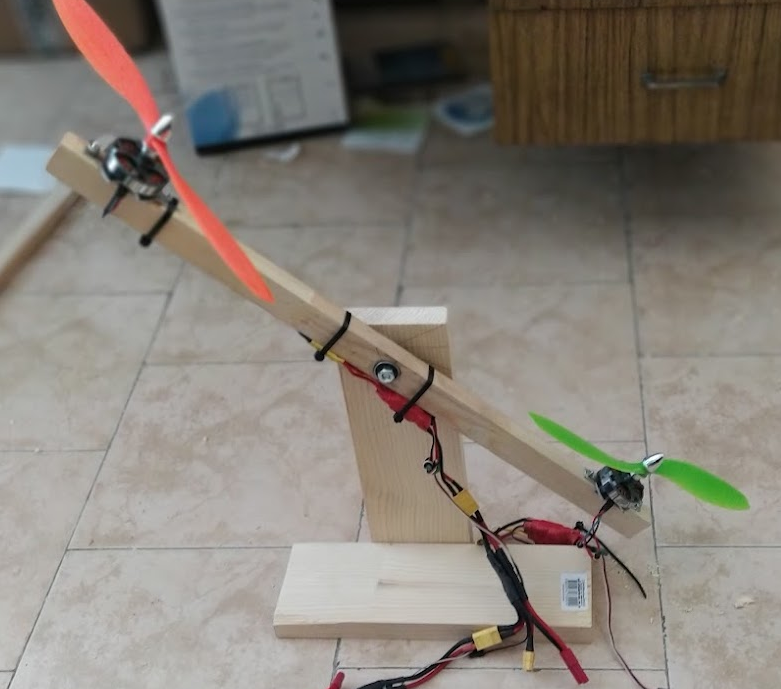
\includegraphics[width=0.7\textwidth]{balance_construction}
    \caption{Конструкция на платформата за управление на ъгъл}
    \label{fig:balance_construction}
\end{figure}

\FloatBarrier





\section{Изграждане на системата и решени проблеми}

\subsection{Изграждане на работната среда}

Голямо количество усилия бяха положени за изграждането на работанта среда, поради решението да не се използват готови решения,
както и поради нуждата от работа под Linux, тъй като множеството от решения имат целева система Windows.

\subsubsection{Система за изграждане (Make)}

Работната среда е изградена на база \textit{Make} което ни позволява да изградим собствен инструментариум за целите на проекта.
\textit{Make} използва на цели (Targets) и взаимовръзките, които изграждат целите (Dependencies). За всяка цел се изгражда дърво
на зависимостите, като се проверява,
кои зависимости имат нужда от преправяне. \textit{Make} е платформно независима и може лесно да бъде пренесена на почти всяка система.
Единственото нещо от което се нуждае \textit{Make} е описание статично или динамично строго описание на взаимовръзките и начините да се
премине от зависимостите към целите. Това става, чрез дефиниране на командни скриптове, което налага ограничението на средата да бъде
достъпна чрез команден интерфейс.

\subsubsection{Компилатор}

Подбраният комилатор е \textit{GCC ARM NON-EABI}, тъй катое платформно независим комилатор с целева крайна система ARM.
комилаторът е конфигуриран през командният интерфейс при извикването си от \textit{Make},
като конфигурацията е публикувана \autoref{lst:make_config}.
конфигурацията включва използването на хардуерният модул за обработка на числа с плаваща запетая,
изключване на всички оптимизации, които комилаторът прави за подобряване на скоростта и използването на паметта с цел гаранция на изпълнението.

\subsubsection{Програматор}

Подбран е командният пакет за \textit{ST-LINK}, тъй като е платформно независим и позволява командно управление на \textit{ST-LINK V2} устройството,
кето е част от комплекта \textit{32F429IDISCOVERY}. Този пакет позволява презаписване на вътрешната флаш памент на конторлера,
както и стартиране и управление на порт за дебък, който да бъде използван за дебъгера.


\subsubsection{Дебъгер}

Подбран е дебъгер GDB, тъй като е платформно независим и позволява командно базирано дебъгване през дебъг порта отворен с помощта на \textit{ST-LINK}.
Дебъгера позволява условно и безусловно поставяне на Breakpoints на отделни моменти от изпълнението, като се използва генерираният \textit{*.elf} обект,
който е записан в флаш паметта на процесора.

\subsubsection{Получаване и обработка на данни}

Данните се изпращат от микроконтролера, през USART порта и се получават на локалната машина (Linux) използвайки TTL четец, \textit{picocom}.
Данните се записват в \textit{*.log} файл, който се обработва автоматично през дефинираната поточна линия от процеси, като създава \textit{*.csv} файл,
който ще бъде използван от \textit{MATLAB (for Linux)} за обработка на данните и генериране на графики.


\subsubsection{Линкерен скрипт}

Написан е линкерен скрипт, който дефинира правилното разположение на паментта на
контролера и управялва разположението и подравняването на символите и секциите в паметта на микроконтролера.
Линкерният скрипт поставя всички констани символи в флаш паметта на контролера, което гарантира че те няма да бъдат променяни.
Линкерният скрипт също гарантира правилното разположение на вектора на прекъсванията в паметта.
Линкерният скрипт отстранява всички символи свързани с стандартните библиотеки, 
тъй като стандартните библиотеки преполагат наличието на операционна система, 
която да имплементира подфункциите, по този начин софтуерът, който пишем е зависим единствено и само на източниците, които ние сме добавили.
Крайният резултат е независим статично линкнат обект, който ще бъде поставен в микроконтролера.


\subsection{Платка за свързване на компонентите}

Като част от проекта е създадена платка, която осъществява връзката между отделните компоненти.
Платката има за цел също да предотврати проблемите възникващи от използването на хардуер работещ на различни
нива на напрежение. 

Пиновете на микроконтролера са толерантни на 5V напрежение само при режим на логическо четене и изходен режим Open-drain.

5V входовете на приемника са директно свързани с пинове тъй като са толерантни на 5V напрежение.
PA0(TIM5 канал 1), PA3(TIM5 канал 4),
PB0(TIM3 канал 3),  PB1(TIM3 канал 4), 
PB4(TIM3 канал 2), PB5(TIM3 канал 1)

За I2C са използвани пинове PA8 (I2C3 SCL) и PA9 (I2C3 SDA),
които са конфигурирани като Open-drain по спецификация.
Те се свързват със сензорната платка, която има собствени Pull-Up резистори.

Пинове PB6(USART1 TX) и PB7 (USART1 RX) се свързват към
UART към USB устройството, което е конфигурирано за вход и изход (3.3V).

За управление на моторите са използвани пинове PD12 - PD15. 
Тъй като за управлението на моторите са нужни 5V тези пинове са конфигурирани в режим Opne-Drain.
Като за запазване на вътрешните Pull-up резистори на контролера са подбрани \cite{pull_up} 
10\(k\Omega\) резистори.

Захранването се черпи от батерията през един от портовете на ESC контролерите, като останалите не са свързани за да се предотвратят проблеми с захранването.



\begin{figure}[htpb!]
    \centering
    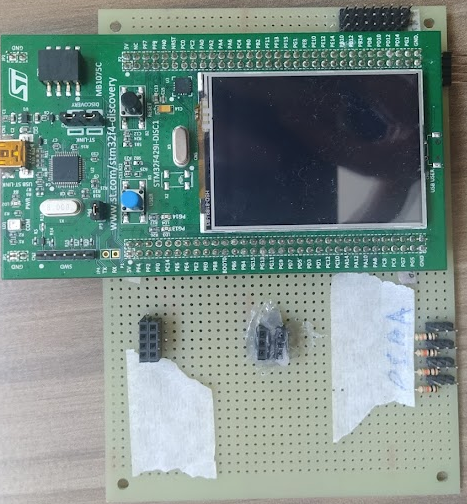
\includegraphics[width=0.7\textwidth]{pcb2}
    \caption{Предна страна на платката}
    \label{fig:pnb_f}
\end{figure}

\begin{figure}[htpb!]
    \centering
    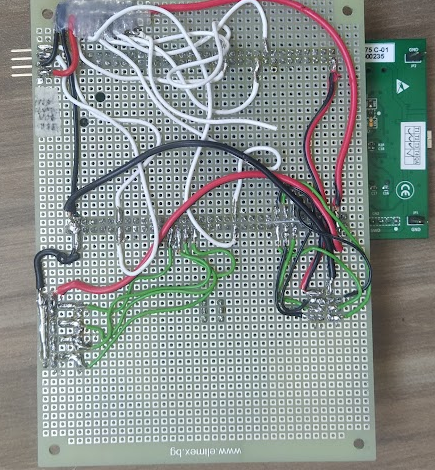
\includegraphics[width=0.7\textwidth]{pcb1}
    \caption{Задна страна на платката}
    \label{fig:pcb_b}
\end{figure}


\subsection{Конфигурация на микроконтролера}

\subsubsection{Стартиране }

Написан е прост стартиращ скрипт на ARM assembly за целите на проекта, който инициализира SP на процесора и инициализира PC=Resethandler.
Скриптът дефинира символите от таблицата за прекъсванията, като .weak референции, към DefaultHandler, който изпълнява безкраен празен цикъл.
Този скрипт има за цел да инициализира .bss секцията на контролера,
както и всички статични променливи, като използва позициите, генерирани от линкерния скрипт, както и да извика функцията за системна инициализация, след което се извиква main финкцията.

\subsubsection{Системна инициализация}

В тази фаза се налага да бъде инициализиран системният часовник.
В нашия случай ще инициализираме системния часовник от високочестотният външен осцилатор (HSE). 
Тъй като при стартиране се използва високочестотният вътрешен осцилатор (HSI), който е
неточен и може да доведе до синхроннизационни проблеми при асинхронни комуникации 
с висок baud-rate като UART.
Поради тази причина се налага инициализирането на системния часовник с времева основа
високочестотният външен осцилатор (HSE), тъй-като е много по прецизен.
Високочестотният външен осцилатор (HSE) на платката е с честота 8MHz, затова използваме
хардуерният PLL модул за увеличаване на честотата със следните настройки:
\begin{verbatim}
    (PLL_M=8, PLL_N=336, PLL_P=2, PLL_Q=7)
\end{verbatim}
, като така получаваме  168MHz честота на системния часовник.
След това инициализираме делителите на честота за отделните шини:
\begin{verbatim}
    (AHB_Prescaler=1, APB1_Prescaler=4, APB2_Prescaler=2).
\end{verbatim}
След настройката на часовниците получаваме следните честоти за отделните шини (\autoref{fig:frequencies})

\begin{figure}[htpb!]
    \centering
    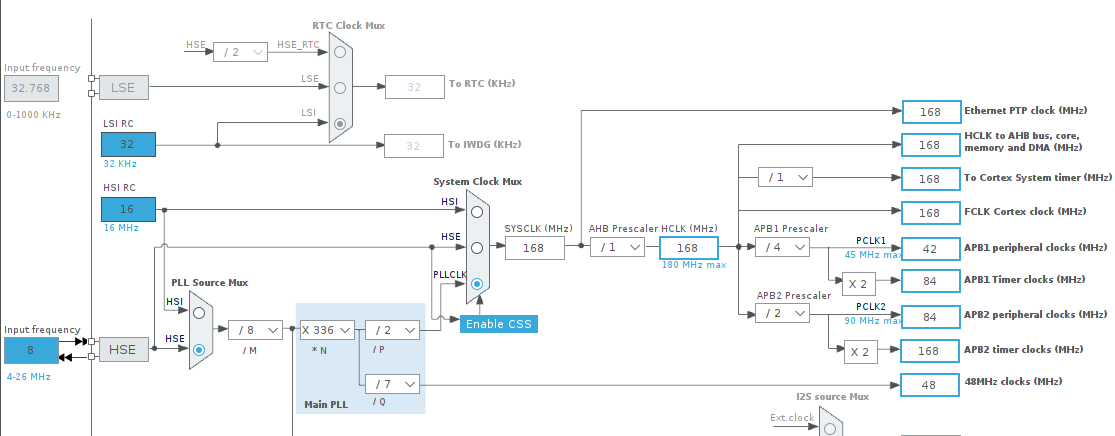
\includegraphics[width=0.9\textwidth]{frequencies}
    \caption{Честоти на системните шини и часовници след конфигурация}
    \label{fig:frequencies}
\end{figure}

Дуга основна част на системанта инициализация е инициализирането на хардуерния модул за числа с плаваща запетая (FPU).
Тъй като от конфигурацията (\autoref{lst:make_config}) настройваме комилатора за работа с модула за числа с плаваща запетая, е важно
преди която и да е операция с числа с плаваща запетая този модул да бъде инициализиран.
Необходимо е инициализацията на FPU да се случи преди преминването в ограничен режим.
Инициализацията се случва, чрез блокът от код (\autoref{lst:enable_fpu}).
\begin{lstlisting}[language=c, caption={Инициализация на модула за числа с плаваща запетая}, label={lst:enable_fpu}]
    /* Enable The FPU*/
    uint32_t* CPACR = (uint32_t*)0xE000ED88;
    *CPACR |=  0b00000000111100000000000000000000;
\end{lstlisting}

\subsubsection{Инициализация на периферията}

\change{WRITE}





\subsection{Моделиране}

\subsubsection{Моделиране на тяга от витло и мотор}

За моделиране на мотора и витлото е приет опростеният модел, който моделира системата като коефициент на усливане и нискочестотен филтър.

\begin{figure}[htpb!]
    \centering
    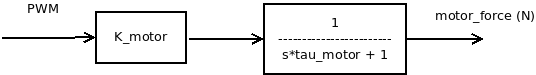
\includegraphics[width=0.7\textwidth]{motor_model}
    \caption{Опростен модел на витло и мотор}
    \label{fig:motor_model}
\end{figure}

\begin{equation}
    G_{motor}(s) = \frac{k_{motor}}{s \tau_{motor} + 1}
    \label{eqn:motor_model}
\end{equation}

Този модел не е добра апроксимация на тягата на моторите,
защото реалната характеристика е нелинейна и се променя спрямо множество параметри (напрежение на батерията, температура, налягане, вляжност, скорост),
но за целите на проекта, т.е. в неголеми времеви интервали и неголеми промени във входния сигнал статичната характеристика
може да бъде описана достатъчно добре, чрез линейната апроксимация (\autoref{eqn:motor_model}).


\subsubsection{Моделиране на платформа за управление на ъгъл на завъртане}

За моделиране на платформата за управление на ъгъл на завъртане (\autoref{fig:balance_force_diagram})
нека приемем, че въртящата час е пренебрежимо тънка, с дължина \(l\), и има маса \(M\). 
Ъгълът, който въртящата част сключва с хоризонта е означен с \(\phi\).
Във края на рамената се намират безчетковите мотори и витлата, моделирани, като концентрирани
маси с големина \(m\), като всеки от тях има сила на тягата означена с \(F_1, F_2\) респективно.
Триенето с въртящата ос е моделирано с коефициентът на триене \(C\).

\begin{figure}[htpb!]
    \centering
    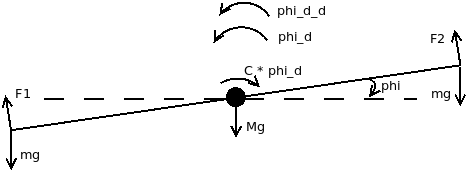
\includegraphics[width=0.7\textwidth]{balance_force_diagram}
    \caption{Диаграма на платформа за управление на ъгъл на завъртане}
    \label{fig:balance_force_diagram}
\end{figure}

От втори закон на Нютон \autoref{eqn:newton1}, 
\begin{equation}
    I \ddot{\phi} = \sum_i \tau_i
    \label{eqn:newton1}
\end{equation}
От където следва:
\begin{equation}
    I \ddot{\phi} = F_2*\frac{l}{2} - F_1*\frac{l}{2} - C \dot{\phi}
    \label{eqn:newton1_expand}
\end{equation}
Нека:
\begin{equation}
    F_2 = F_0 + \delta f, F_1 = F_0 - \delta f 
\end{equation}
След като заместим в \autoref{eqn:newton1_expand}
\begin{equation}
    I \ddot{\phi} = (F_0 + \delta f)*\frac{l}{2} - (F_0 - \delta f)*\frac{l}{2} - C \dot{\phi}
\end{equation}
Плучаваме:
\begin{equation}
    I \ddot{\phi} + C \dot{\phi} = l * \delta f
\end{equation}
Което опростява системата до линейна SISO система.

Апроксимираме инерционният момент \(I\) като :
\begin{align}
    I &= I_{rod} + 2*I_{motor}\\
    I &= \frac{1}{12}Ml^2 + 2m(\frac{l}{2})^2 \\
    I &= \frac{l^2}{12}(M + 6m)
\end{align}

При нулеви начални условия след трансформация на Лаплас получаваме:
\begin{equation}
    s^2 I \bar{\Phi}(s) + s C \bar{\Phi}(s) = l * \bar{\delta f}(s) 
\end{equation}
От където получаваме предавателната функция:
\begin{equation}
    G_{platform}(s) = \frac{\bar{\Phi}(s)}{\bar{\delta f }(s)} = \frac{l}{s ( s I + C)}
\end{equation}

За получаване на предавателната функция на отворената система:
\begin{equation}
    G_{sys} = G_{motor}(s)G_{platform}(s) = 
    \frac{k_{motor} l}{s( s I + C)(s \tau_{motor} + 1)} 
\end{equation}


\subsubsection{Моделиране на платформа с 4 ротора}

\FloatBarrier
Безполитните летателни платформи с 4 ротора се разделят на 2 основни дизайна "+" и "х". 
Х-конфигурацията се счита за по-стабилна, от колкото + конфигурацята.

Рамката на платформата се състои от 2 кръстосани рамена, като роторите са монтирани в краищата им.
Роторите на всяко рамо се въртят в противоположни посоки както е показано на фигура\ref{fig:rotors}
Важно е да се отбележи, че перките на ротори 1 и 3 имат обратен наклон  спрямо перките на роторите 2 и 4.
Така тягата на всияки ротори е в еднаква посока. Респективно различната посока на въртене на роторите е нужна
за да може приведеният въртящ момент да бъде равен на нула, за да може платформата да запазва своята ориентация.

\begin{figure}[!h]
	\centering
	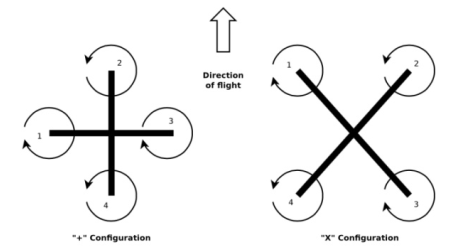
\includegraphics[width=0.6\columnwidth]{rotors}
	\caption{Основни типове на конфигурация .}
	\label{fig:rotors}
\end{figure}


Тук е важно да дефинираме 2 основни координатни системи, които ще използваме. 
Първата е спрямо земята (XE,YE,ZE)  а втората е спрямо тялото на квадракоптера (XB,YB,ZB).
Ориентацията на квадракоптера може да се дефинира чрез Ойлеровите ъгли на тялото на квадракоптера.
На фигура\ref{fig:kinematika} са показани коростите на въртене на роторите \( \omega_1 , \omega_2 ,
\omega_3 , \omega_4 \), силите на тягата генерирана от перките \(T_1,T_2,T_3,T_4\).

Позицията на квадракоптера е дефинирана, в координатната система спрямо земята по осите x,y,z с вектора 
\(\xi = [x,y,z]^T\). А ориентацията се дава, чрез Ойлеровите ъгли \(\eta = [\phi,\theta,\psi]^T\).
А векторът \(q = [\xi,\eta]^T\) съдържа както се вижа и линейлите и ъгловите кооргинати.

Центъра на масите на дрона се смята за основа на координатната система на тялото на дрона. Спямо тялото на дрона
линейните скорости се определят от \(JB = \begin{bmatrix}Jx,B\\Jy,B\\Jz,B\end{bmatrix}\) а ъгловите скорости се
определят от \(\omega = \begin{bmatrix}p\\q\\r \end{bmatrix}\)

\begin{figure}[!h]
    \centering
    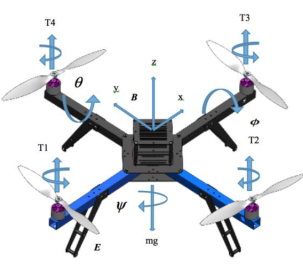
\includegraphics[width=0.6\columnwidth]{kinematika}
    \caption{Сили, моменти и отправни системи на квадракоптера}
    \label{fig:kinematika}
\end{figure}

За да може квадракоптерът да се носи във въздуха е нужно да са спазени следните условия:

\begin{align}
		\sum_{i=1}^{4} T_i  =& -mg \\
		\sum_{i=1}^{4} M_i  =& 0 \\
		T_{1,2,3,4} ||& g \\
		( \omega_1 + \omega_3 ) - ( \omega_2 + \omega_4 ) =& 0 
\end{align}

от което и следва, че \(\phi=0,\theta=0,\psi=0\).

При увеличаване/намаляване на скоростта на роторите дронът може да се движи, нагоре и надолу.
За да се движим нагоре : \(\sum_{i=1}^4 T_i > -mg\).
И респективно да се двиим надолу: \(\sum_{i=1}^4 T_i < -mg\). Като не забравяме, 
че и в двата случая другите параметри остават незасегнати.

За промяна на ориентацията се налага да:
\begin{align}
		\dot{\psi} = k_{\psi}((\omega_1+\omega_3)-(\omega_2 + \omega_4)) ,& \psi = \int \dot{\psi}dt\\
		\dot{\phi} = k_{\phi}((\omega_1 + \omega_4) - (\omega_2+\omega_3 )) ,& \phi = \int \dot{\phi}dt\\
		\dot{\theta} = k_{\theta}((\omega_1+\omega_2) - (\omega_3 +\omega_4)) ,& \theta = \int \dot{\theta}dt
\end{align}


От което следва, че при намаляне на скоростта на ротор 2 и уваличаване на скоростта на ротор 4 постигаме
завъртане по \(\phi\). Съответно намаляване на скоростта на ротор 1 и увеличаване на скоростта на ротор 3 
постигаме завъртане по \(\theta\)  и съответно намаляване на скоростта на срещуположни ротори и съотетно увеличаване на другите два посигаме завъртане по \(\psi\).

\begin{figure}[!h]
    \centering
    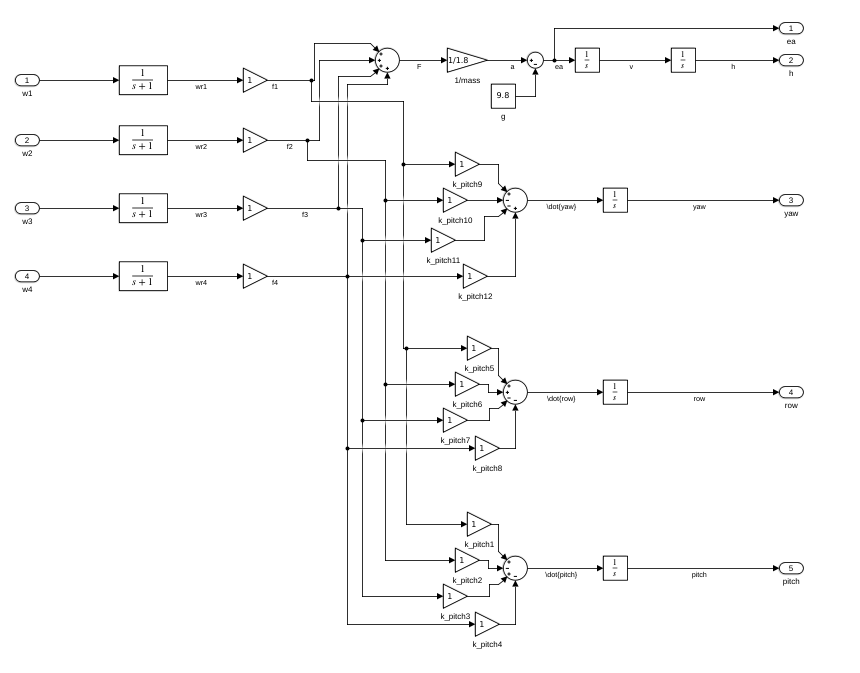
\includegraphics[width=0.8\columnwidth]{quadrotor_simulink}
    \caption{SIMULINK схема на динамиката на платформа с 4 ротора.}
    \label{fig:quadrotor_simulink}
\end{figure}


\FloatBarrier


\subsection{Компенсация на сензорни отмествания}

\subsubsection{Компенсация на жироскопен дрейф}
\FloatBarrier
Жироскопите обикновено не са силно зашумени за разлика от
акселерометрите, но имат своите недсостатъци.
Основен проблем при жироскопите е т.нар. жироскопен дрейф.
В неподвижно състояние жироскопът показва малко постоянно завъртане в някоя посока.
Жироскопният дрейф зависи основно от температурата.

За да калибрираме и занулим стойностите на жироскопа
се налага да направим полиномиална компенсация по температура.

За целта жироскопа е ухладен до \(0^{\circ}C\)
след което е поставен неподвижно бавно да се загрее в продължение на 45мин до стайна температура.
През цялото време събираме данните от жироскопа и измерената от бордовия термометър температура.
След приключване на експеримента използваме матлаб за намиране на полином,
който точно описва получените данни за всяка от осите.

\begin{figure}[htpb!]
    \centering
    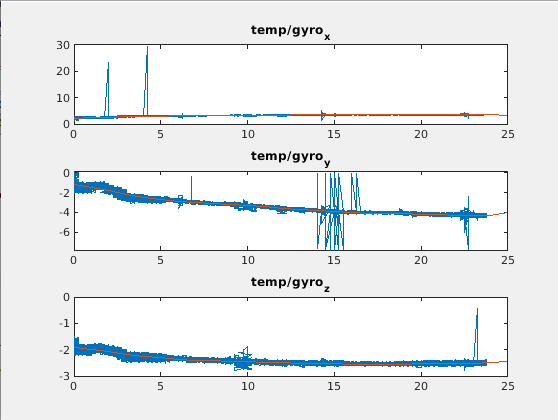
\includegraphics[width=0.9\textwidth]{gyro_drift_calibrate}
    \caption{Жироскопен дрейф спрямо температура и полиномиална компенсация спрямо температура}
    \label{fig:gyro_drift_calibrate}
\end{figure}

\begin{lstlisting}[language=matlab, caption={Получени полиноми за коменсация на жироскопният дрейф}, label={lst:gyro_drift_poly}]

    p_x =

     -42.6978e-9  3.7797e-6  -131.8066e-006  2.2717e-3  -19.5918e-3  67.9744e-3  95.1384e-3  2.2440e+0

  p_y =
  
      87.1716e-9  -7.6384e-6  263.1019e-006  -4.4660e-3  37.8030e-3  -129.2365e-3  -191.6577e-3  -1.1695e+0
  p_z =
  
      15.9591e-9  -1.4613e-6  53.0721e-006  -961.5439e-6  8.8365e-3  -33.3197e-3  -44.0584e-003  -1.9076e+0

\end{lstlisting}


\FloatBarrier


\subsubsection{Компенсация на магнитни отмествания от околната среда}
\FloatBarrier
Магнитометрите имат постоянно отместване поради средата в която се намират.
Това отместване се дължи на металните и магнитни обекти,
както и всички електромагнитни смущения причинени от заобикалящата ни среда.
Поради факта, че в близката ни околна среда тези смущения са постоянни, което означава, че ние можем да ги компенсираме статично.


За целта поставяме сензора в нормална позиция и бавно го завъртаме, като се стараем да покрием възможно най-много ъглови комбинации.
След получаване на данните виждаме, че те образуват Елипсоид с отместен център.
Използваме техника на Мерайо.
Идентифицираме елипсоида и отместването на центъра,
след което правим трансформация елипсоид-сфера,
след което изваждаме отместването на центъра.
Верифицираме резултатът, като виждаме, че всички измерени точки са в допостим диапазон от повърхността на сфера с център 0 и радиус 1.

\begin{figure}[htpb!]
    \centering
    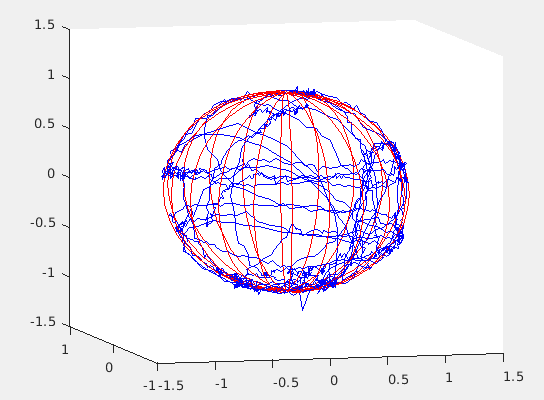
\includegraphics[width=0.9\textwidth]{mag_calibration}
    \caption{Компенсирани данни получени от магнитометър}
    \label{fig:mag_calibration}
\end{figure}

\begin{lstlisting}[language=matlab, caption={Получени трансформация елипсоид-сфера и отместване на център}, label={lst:mag_cal_trans}]

    U =

    21.4229e+000   837.9000e-003     3.0861e+000
     0.0000e+000    21.6201e+000     2.0207e+000
     0.0000e+000     0.0000e+000    27.2441e+000

    c =

    -1.6000e-003
    19.9000e-003
    45.7000e-003

\end{lstlisting}


\subsection{Калманов наблюдаел}

Калмановият наблюдател е рекурсивен естиматор на 
състоянието на системата, който дава статистически
оптимална естимация на състоянието дори и при използване на
зашумени входни данни.
Калмановият филтър често се използва при т.нар сензорно сливане,
и е най-честият метод, който се използва 
за обединяване на жироскоп и акселерометър за намиране на ориентация.
Калмановият филтър може да бъде разделен на 2 основни стъпки: предсказване и обновяване.

В стъпка предсказване алгоритъма продуцира оценка за състоянието, както и за неопределеностите в състоянието,
в резултат на шум. Тази стъпка може да бъде изпълнена множество пъти, като предсказанието е все по-неопределеност с всяка итерация.
В стъпка обновяване алгоритъма сравнява предсказанията спрямо зашумените измервания и обновява
оценката използвайки претеглена комбинация 
от предсказание и измерване, като се дава по-високо
тегло на оценкитв с по-ниска неопределеност.

Алгоритъма може да бъде изпълняван на всяка итерация,
без нужда от стари стойности на използваните променливи.

Крайната естимация може да бъде описана като оптимално решение,
коато системата е линейна и е зашумента от шум в състоянията и шумове от измерванията с Бял Гаусов Шум.
Можем да представим това математически чрез модел на предсказанието 
и модел на измерването.

\begin{align}
    x_k = F x_{k-1} + B u_k + N(0, Q_k) \\
    z_k = H x + N(0, R_k)
\end{align}

Филтърът ще бъде използван за оценка на ойлеровите ъгли, на завъртане спрямо оста X и оста Y.
Така дефинираме вектор на състоянията във форма:
\begin{equation*}
    x = 
    \begin{bmatrix}
        \phi\\
        \psi\\
        \omega_{xb}\\
        \omega_{yb}
    \end{bmatrix}_k
\end{equation*}

Моделите на измерване и предсказване са дефинирани:
\begin{align}
    \begin{bmatrix}
        \phi\\
        \psi\\
        \omega_{xb}\\
        \omega_{yb}
    \end{bmatrix}_k &=
    \begin{bmatrix}
        1 & 0 & -d_t & 0 \\
        0 & 1 & 0 & -d_t \\
        0 & 0 & 1 & 0 \\
        0 & 0 & 0 & 1
    \end{bmatrix}_k *
    \begin{bmatrix}
        \phi\\
        \psi\\
        \omega_{xb}\\
        \omega_{yb}\\
    \end{bmatrix}_{k-1}
    +
    \begin{bmatrix}
        d_t & 0 & 0 & 0 \\
        0 & d_t & 0 & 0 \\
        0 & 0 & 0 & 0   \\
        0 & 0 & 0 & 0
    \end{bmatrix}_k *
    \begin{bmatrix}
        \omega_{x}\\
        \omega_{y}\\
        0 \\
        0
    \end{bmatrix}_{k}
    +
    N(0, Q_k) \\
    \begin{bmatrix}
        A_\phi\\
        A_\psi\\
        0\\
        0
    \end{bmatrix}_k &=
    \begin{bmatrix}
        1 & 0 & 0 & 0 \\
        0 & 1 & 0 & 0 \\
        0 & 0 & 0 & 0 \\
        0 & 0 & 0 & 0
    \end{bmatrix}_k *
    \begin{bmatrix}
        \phi\\
        \psi\\
        \omega_{xb}\\
        \omega_{yb}\\
    \end{bmatrix}_{k}
    +
    N(0,R_k)
\end{align}

След снемане на експериментални данни са под брани следните
ковариантни матрици:

\begin{align}
    Q =
    \begin{bmatrix}
        33.8 & 0 & 0 & 0 \\
        0 & 33.8 & 0 & 0 \\
        0 & 0 & 0.4 & 0 \\
        0 & 0 & 0 & 0.4
    \end{bmatrix} &,&
    R = \begin{bmatrix}
        32 & 0 & 0 & 0 \\
        0 & 32 & 0 & 0 \\
        0 & 0 & 0 & 0 \\
        0 & 0 & 0 & 0
    \end{bmatrix}
\end{align}

Така синтезирания филтър на Калман е имплемнтиран в контролера.
За проверка на филтъра е изпълнен следният експеримент.
След стартиране изчакваме, за да сме сигурни, че филтърът се е устнановил.
След което накланяме ръчно дрона под ъгъл около \(20^{\circ}\), 
като задържаме ъгъла за няколко секунди поставяме в 
изходно положение отново за няколко секунди,
след което повтаряме наклона в обратната посока и отново задържаме.
Връщаме в изходна позиция изчакваме, след което внасяме допълнителни смущения в системата,
чрез относително силни почувкания в успореднин на на осите на въртене.

Резултатите от експеримента могат да бъдат проверени в (\autoref{fig:kalman_filter_time_vs_raw}, \autoref{fig:kalman_filter_time_vs_raw2})

\begin{figure}[htpb!]
    \centering
    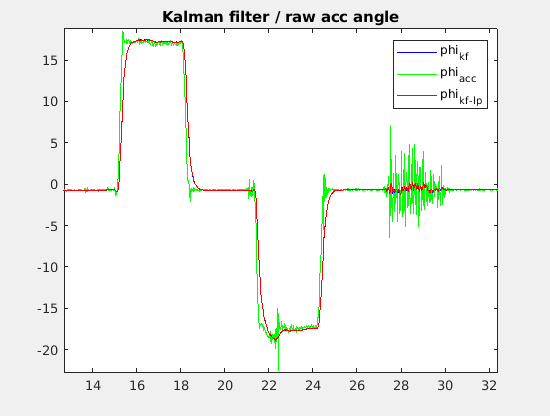
\includegraphics[width=0.8\textwidth]{kalman_filter_time_vs_raw}
    \caption{Проверка на Калман филтъра за ос \(\phi\)}
    \label{fig:kalman_filter_time_vs_raw}
\end{figure}

\begin{figure}[htpb!]
    \centering
    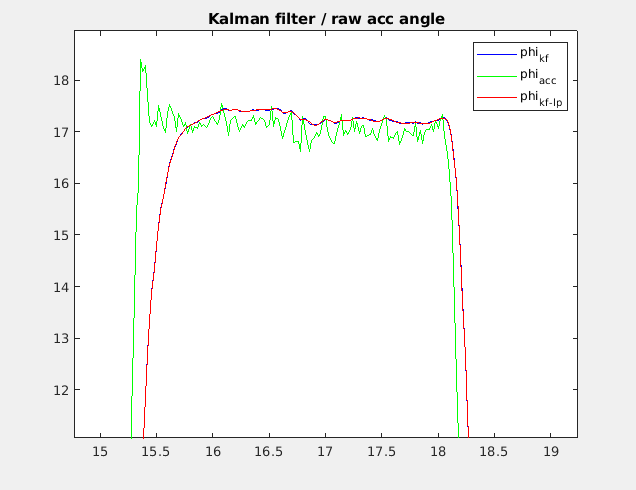
\includegraphics[width=0.8\textwidth]{kalman_filter_time_vs_raw_2}
    \caption{Проверка на Калман филтъра за ос \(\phi\), приближен}
    \label{fig:kalman_filter_time_vs_raw2}
\end{figure}

Забелязваме, че филтъра успешно потиска смущенията и крайният резултат се установява за около \(0.1s\).

\FloatBarrier

\subsection{Експериментални задачи}

\subsubsection{Снемане на статичните характеристики за тягата на мотор с витло}

Характеристиките са снети при използване на напълно заредена батерия.
Процедурата по снемане е както следва:
Използвана е платформата за управление на ъгъл на завъртане,
като под рамо едно е поставена везна. Върху везната се поставя право парче дърво, което да се допира във въртящата част на платформата,
на разстояние от центъра равно на разстоянието на срещуположният двигател от центъра. 
По този начин предаването на сила е 1:1.
Кантара се занулява и се задават управляващи сигнали в диапазона \(950 \to 1950ms\) запълване,
на ШИМ \(50Hz\). при подаването на всеки сигнал се изчаква преходните процеси да преминат и се снема стойността от везната.

\begin{figure}[htpb!]
    \centering
    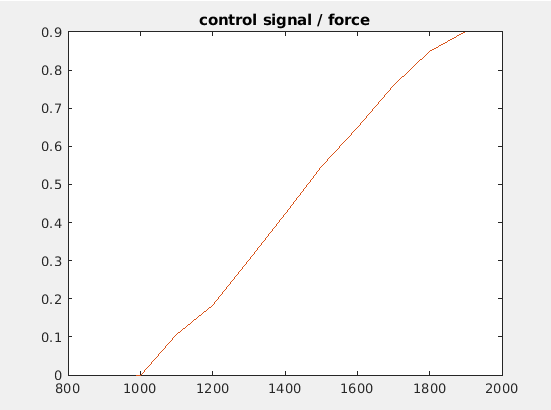
\includegraphics[width=0.7\textwidth]{control_force}
    \caption{Управляващ сигнал / тяга}
    \label{fig:control_force}
\end{figure}

След снемане на характеристиките е изчкислен предавателен коефициент \(k_{motor=1.21e-3}\) в диапазона на управление (\(1300\to1700\)).
Важно е, че характеристиката е почти линейна в диапазона на управление.









\section{Предложения за надграждане}

При експериментирането с платформата бе забелязано,
че металните профили не потискат добре вибрациите, което създава силни зашумявания в акселерометъра.
Това не се наблюдава в повечето готови решения от подобен размер поради използването на карбонови профили.

За подобряване на стабилността и качеството на управлението се предлага използване на по-високи честоти за измерванията,
както и използване на контролери за управление с дигитален вход за  скоростта на моторите,
тъй като използването на ШИМ не е надеждно за точно задаване на скоростта.

За момента този труд се фокусира върху управлението на ъгъл на завъртане, като един от основните проблеми за цялостно изграждане на беезпилотна платформа с четири ротора.
Като надграждане на този труд се предлага интегрирането на управление по височина, като може да бъде използвано сензорно сливане на сензор за разстояние, и барометър.
Както и използването на GPS и камера за управление чрез позициониране в пространството.

\section{Заключение}

Като част от този труд бяха решени множество иженерни по отношение на създаването на цялостна работна среда за разработка на
софтуер за вградени системи с микроконтролери от семейство STM32M4xxx.

Бяха изградени и/или модифицирани множество библиотеки за математическа обработка с цел изясняване на математическите процедури,
които изграждат често използваните с цел управление алгоритми.

При създаване на системата бе инициализиран хардуера, и бяха инициализирани всички сензори, като често се оказваше,
че документацията на отделните компоненти е недостатъчна и/или непълна.

При създаването на платката за свързване на компонентите бяха решени множество инженерни проблеми свързани с използването на
различни напрежитлни нива на различните компоненти както и коректното разпределение на пиновете на конролета, тъй-като 
микрочипа е част от платка за оценка на функционалностите бе нужно пулно изчитане и сравнение на документацията на платката и контролера,
както и множество от експериментални проверки на изходите за да се гарантира, че пподкачената допълнителна периферия няма да създава проблеми
при комуникацията и четенето на данни.

Като часто от проекта бяха написани драйвъри както и манипулатори (handlers) на прекъсванията с цел възстановяване при
неблагоприятни състояния и грешки в комуникацията. Това намалява аварийните ситуации в случай на грешки.

За сензорите са синтезирани компенсации на слущенията, като са използвани експериментално снети данни.
Синтезиран е филтър на калман, който е използван за оценка на ъгъла на завъртане.

Изградена е платформа за управление на ъгъл на завъртане. Изведен е теоретичен модел на роторите, както и на платформата.
Идентифицирани са параметрите на модела, след което е синтезирано управление.


\newpage
\section{Литература}

\nocite{*}
%\printbibliography[keyword=bg]
%\printbibliography[keyword=en, heading=none]
%\printbibliography[notkeyword=bg, notkeyword=en, heading=none]
\printbibliography[heading=none]


\newpage
\section*{Приложения}

\begin{appendix}
    \section{Системна конфигурация}

    \lstinputlisting[language=make, caption={\texttt{config.mk}}, label={lst:make_config}]{src/config.mk}

    \section{Процедура за изчисляване на магнитометърна компенсация}
    \lstinputlisting[language=matlab, caption={\texttt{MgnCalibration.mk}}, label={lst:make_config}]{src/MgnCalibration.m}
\end{appendix}

\end{document}
